\chapter{Tổng quan lý thuyết}
\label{Chapter2}

\section{Hệ thống Federated Learning}

\codeword{#todo: ứng dụng của FL?}

\subsection{Định nghĩa}

\textbf{Định nghĩa về FL} \cite{yang2019federated}: Giả sử có $n$ máy khách, máy khách thứ $i$ ký hiệu là $c_i$ $(i\in [1, n])$, chứa tập dữ liệu $\mathcal{D}_i$. FL là một quá trình học mà ở đó, các chủ sở hữu dữ liệu (ở đây có thể hiểu là các thiết bị biên) cùng hợp tác huấn luyện một mô hình $\mathcal{M}$ và đạt được độ chính xác $f$ nhưng không có bất kỳ chủ sở hữu dữ liệu $c_i$ nào chia sẻ tập dữ liệu $\mathcal{D}_i$ của chúng.

Gọi $\bar{\mathcal{M}}$ là mô hình máy học được huấn luyện trên tập dữ liệu $\mathcal{D}  = \mathcal{D}_1 \cup \mathcal{D}_2 \cup ... \cup \mathcal{D}_n$ và cho độ chính xác $\bar{f}$. $f$ và $\bar{f}$ chỉ được phép chênh lệch nhau một khoảng nhỏ. Gọi $\delta$ là một giá trị thực không âm, nếu $\mid f-\bar{f}\mid < \delta$ ta nói mô hình $\mathcal{M}$ có \textit{$\delta$ - accuracy loss}.

\textbf{Định nghĩa về tính hợp lệ} \cite{li2021survey}: Ký hiệu $\mathcal{M}_i$ là mô hình được huấn luyện trên tập dữ liệu $\mathcal{D}_i$ và cho độ chính xác $f_i$. Mô hình $\mathcal{M}$ được gọi là hợp lệ nếu tồn tại $i\in [1,n]$ sao cho $f>f_i$.

\subsection{Một hệ thống Federated Learning điển hình}

\textbf{Thành phần và các tương tác trong hệ thống.} Một hệ thống FL (Hình \ref{fig:fl}) thường bao gồm hai thành phần chính: máy chủ (đóng vai trò là đối tượng duy trì mô hình toàn cục) và máy khách (đóng vai trò là đối tượng nắm giữ dữ liệu huấn luyện). Hai thành phần này tương tác với nhau theo ba bước sau \cite{lim2020federated}:

\begin{itemize}
    \item \textit{Khởi tạo.} Máy chủ khởi tạo trọng số $w_G^0$ cho mô hình toàn cục và các siêu tham số cho quá trình huấn luyện. Thông tin này sau đó được gửi đến một tập hợp con các máy khách được chọn để tiến hành huấn luyện.

    \item \textit{Huấn luyện và cập nhật mô hình cục bộ.} Tại bước huấn luyện thứ $t$, máy khách $c_i$ nhận trọng số $w_G^t$ từ máy chủ và tiến hành huấn luyện cục bộ trên tập dữ liệu $\mathcal{D}_i$. Tham số $\theta_i^{t+1}$ thu được sau quá trình huấn luyện (có thể là trọng số $w_i^{t+1}$ hoặc đạo hàm hàm lỗi $g_i^{t+1}$) được máy khách gửi về máy chủ để tổng hợp.

    \item \textit{Tổng hợp và cập nhật mô hình toàn cục.} Máy chủ nhận tham số $\theta_i^{t+1}$ gửi về từ các máy khách được chọn trước đó, tiến hành tổng hợp $w_G^{t+1}$ - trọng số mới của mô hình toàn cục và gửi trọng số này đến một tập hợp con các máy khách khác để bắt đầu bước huấn luyện toàn cục mới.
\end{itemize}

\begin{figure}[H]
    \begin{center}
        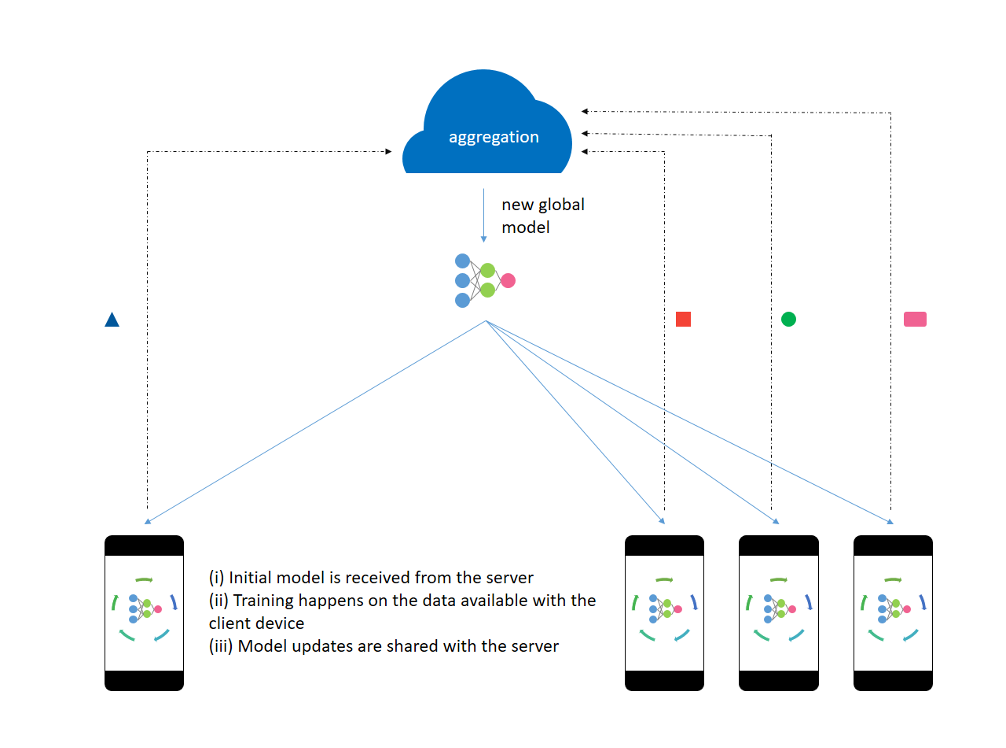
\includegraphics[scale=0.85]{images/fl.png}
        \caption{Hai thành phần chính và quá trình tương tác giữa chúng trong hệ thống FL \cite{chandorikar_2020}}
        \label{fig:fl}
    \end{center}
\end{figure}

Máy chủ sẽ lặp lại bước 2 và bước 3 cho đến khi độ lỗi hội tụ hoặc độ chính xác đạt đến một ngưỡng nhất định. Khi quá trình huấn luyện kết thúc, tham số của mô hình toàn cục sẽ được phân phối đến toàn bộ máy khách trong hệ thống.

\label{purpose_fl}
\textbf{Mục tiêu của hệ thống FL.} Tại đây khảo sát hai mục tiêu của hệ thống FL: (1) - Mục tiêu cục bộ; (2) - Mục tiêu toàn cục.

Các máy khách trong hệ thống hướng đến việc thực hiện mục tiêu cục bộ. Ban đầu, máy khách $c_i$ nhận một trọng số toàn cục $w_G$ từ máy chủ. Máy khách này sau đó sẽ cố gắng tìm kiếm một trọng số $w_i^{t+1}$ giúp cực tiểu hóa hàm lỗi cục bộ. Nói cách khác, $w_i^{t+1}$ phải thỏa mãn thỏa mãn:

\begin{equation}
    \label{eq:opt_client}
    w_i^{t+1} = \arg\min_{w_i}{f_{local}(w_i^t)}
\end{equation}

Trong đó, $f_{local}(w_i)$ là hàm lỗi trên tập dữ liệu của $c_i$. Với $\alpha$ là siêu tham số học cục bộ, $w_{i(j)}$ là trọng số tại bước huấn luyện $j$ của $c_i$, lời giải của phương trình \ref{eq:opt_client} theo phương pháp SGD sau $e$ bước huấn luyện có thể được viết như sau:

\begin{equation}
    \begin{cases}
        w_{i(0)}^t = w_G^t\\
        w_{i(j)}^t = w_{i(j-1)}^t - \alpha \nabla f_{local}(w_{i(j-1)}^t)\\
        w_i^{t+1} = w_{i(e)}^t
    \end{cases}
\end{equation}

Hay:

\begin{dmath}
    w_i^{t+1} \leftarrow w_i^t - \alpha\nabla f_{local}(w_i^t)
\end{dmath}

Mặt khác, mục tiêu toàn cục, cũng là mục tiêu chính của hệ thống FL, được máy chủ thực hiện bằng cách tìm kiếm một trọng số $w_G^*$ giúp tối thiểu hóa hàm lỗi của cả hệ thống \cite{yin2021comprehensive}:

\begin{dmath}
    \label{eq:opt_server}
    w_G^* = \arg \min_{w_G}{f_{global}(w_G)}
        = \arg \min_{w_G}{\frac{1}{n} \sum_{i=1}^n{f_{local}(w_i)}}
\end{dmath}

Trong đó, $f_{global}(w_G)$ là hàm lỗi toàn cục của hệ thống. Để giải phương trình \ref{eq:opt_server}, máy chủ thực hiện tổng hợp tham số gửi về từ máy khách bằng một trong hai cách: lấy trung bình trọng số \parencite{mcmahan2017communication, aono2017privacy, yoon2021fedmix} hoặc lấy trung bình đạo hàm \parencite{chen2018federated, mcmahan2017learning}.

Đặt $n_i = |\mathcal{D}_i|$ là số điểm dữ liệu của tập $\mathcal{D}_i$, $N = \sum_{i=1}^n{n_i}$ là tổng số điểm dữ liệu có trong cả hệ thống. Phương pháp lấy trung bình trọng số tính toán trọng số toàn cục tại bước huấn luyện thứ $t$ từ các trọng số của máy khách như sau \cite{mcmahan2017communication}:

\begin{equation}
    \label{eq:agg_w}
    w_G^{t+1} = \sum_{i=1}^n{\frac{n_i}{N} w_i^{t+1}}
\end{equation}

Trái lại, phương pháp lấy trung bình đạo hàm đòi hỏi máy khách gửi về đạo hàm hàm lỗi sau khi kết thúc quá trình huấn luyện cục bộ. Với $\beta$ là siêu tham số học toàn cục, quá trình tổng hợp tại bước huấn luyện $t$ được biểu diễn theo công thức:

\begin{dmath}
    w_G^{t+1} = w_G^t - \beta  \sum_{i=1}^n{\frac{n_i}{N} \nabla f_{local}(w_i^{t+1})}
        = w_G^t - \beta g^{t+1}
\end{dmath}

Sau khi khảo sát cả hai phương pháp tổng hợp tham số của máy chủ, nghiên cứu \cite{yin2021comprehensive} chỉ ra rằng, việc lấy trung bình trọng số giúp hệ thống có khả năng chịu được việc mất cập nhật, nhưng không đảm bảo việc hội tụ. Trái lại, việc lấy trung bình đạo hàm giúp hệ thống đảm bảo sự hội tụ nhưng tiêu tốn nhiều chi phí truyền tin hơn. Để phù hợp hơn với giới hạn về chi phí giao tiếp và lưu trữ, khóa luận này tổng hợp trọng số toàn cục bằng phương pháp lấy trung bình trọng số.

\textbf{Phân loại hệ thống Federated Learning.} Nghiên cứu \cite{yin2021comprehensive} đề xuất các phân loại các hệ thống FL dựa trên phân bố dữ liệu đầu vào của chúng. Theo đó, ba phân bố dữ liệu: (1) - Phân bố dữ liệu theo chiều ngang (Horizontal data partitioning), (2) - Phân bố dữ liệu theo chiều dọc (Vertical data partitioning), (3) - Phân bố dữ liệu hỗn hợp (Hybrid data partitioning) sẽ ứng với ba loại hệ thống FL (Hình \ref{fig:taxonomy_fl}): (1) - Hệ thống FL theo chiều ngang (Horizontal FL), (2) - Hệ thống FL theo chiều dọc (Vertical FL), (3) - Hệ thống học chuyển giao tri thức (Federated Transfer Learning).

\begin{figure}[H]
    \begin{center}
        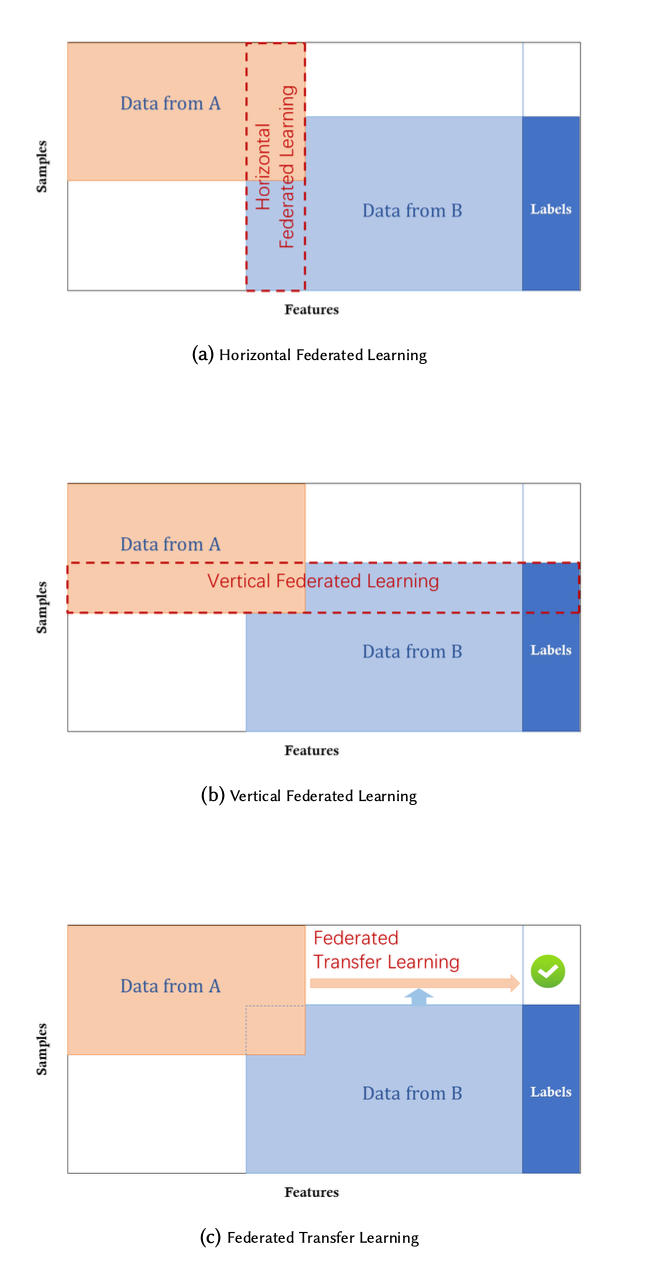
\includegraphics[height=20cm]{images/taxonomy_fl.png}
        \caption{Ba loại hệ thống FL với phân bố dữ liệu tương ứng \cite{yang2019federated}}
        \label{fig:taxonomy_fl}
    \end{center}
\end{figure}

\textit{Hệ thống Horizontal FL.} Phân bố dữ liệu theo chiều ngang là kiểu phân bố dữ liệu mà ở đó các bên tham gia vào hệ thống cùng sở hữu các đặc tính dữ liệu giống nhau nhưng giá trị định danh của mẫu dữ liệu của các bên là khác nhau. Ví dụ, khi các bên tham gia hệ thống là các trường đại học, họ sẽ muốn quản lý các thông tin giống nhau về sinh viên như họ và tên, mã số sinh viên,... Kiến trúc Horizontal FL rất phù hợp để huấn luyện mô hình học tuân theo phân phối này \cite{yin2021comprehensive}.

Dựa vào kiến trúc giao tiếp, có thể chia Horizontal FL ra làm hai loại: Kiến trúc client-server và kiến trúc peer-to-peer (P2P). Kiến trúc client-server, hay còn gọi là kiến trúc FL tập trung, về cơ bản sẽ thực hiện các bước huấn luyện giống như đã trình bày trong phần \textbf{Thành phần và các tương tác trong hệ thống}. Trong khi đó, kiến trúc P2P, hay còn gọi là kiến trúc FL phân tán không có một máy chủ cố định. Tại mỗi bước huấn luyện toàn cục, một máy khách trong hệ thống được chọn làm máy chủ. Quá trình huấn luyện sau đó được thực hiện giống như kiến trúc client-server.

Một hệ thống Horizontal FL thường có số lượng máy khách rất lớn, khả năng lưu trữ và tính toán tại các máy khách không cần quá cao (ví dụ như điện thoại thông minh, máy tính bảng) và tần suất một máy khách tham gia huấn luyện là rất thấp.

\textit{Hệ thống Vertical FL.} Đây là kiến trúc phù hợp với phân bố dữ liệu theo chiều dọc. Trong phân bố dữ liệu dạng này, các bên tham gia hệ thống sở hữu các đặc tính dữ liệu khác nhau nhưng giá trị định danh của mẫu dữ liệu của các bên là giống nhau. Ví dụ, khi các bên tham gia hệ thống là ngân hàng và trường đại học. Với cùng một định danh người dùng, thuộc tính mà ngân hàng và trường đại học lưu trữ là rất khác nhau.

\textit{Hệ thống Federated Transfer Learning.} Khi phân bố dữ liệu của các bên tham gia hệ thống không sở hữu chung các đặc tính dữ liệu hay giá trị định danh của từng mẫu, người ta gọi đây là phân bố dữ liệu hỗn hợp. Ví dụ, khi các bên tham gia hệ thống là một ngân hàng ở Hoa Kỳ và một trường đại học ở Việt Nam. Do cản trở địa lý và nhu cầu quản lý thông tin khác nhau, chủ sở hữu dữ liệu này sẽ không có chung thuộc tính hay giá trị định danh nào. Trong trường hợp này, FTL có thể được sử dụng để chuyển giao tri thức giữa các bên tham gia.

Dựa vào các đặc điểm phân loại nêu trên, \textbf{hệ thống FL trong khóa luận này được xếp vào nhóm hệ thống Horizontal FL tập trung, bao gồm một máy chủ quản lý nhiều máy khách}.

\section{Khảo sát dữ liệu Non-IID}

Dữ liệu tại các máy khách thường được sinh ra dựa trên nhu cầu của người dùng cuối. Do đó, loại dữ liệu này thường có tính cá nhân hóa cao và không đồng nhất. Thuật ngữ sử dụng để chỉ phân phối dữ liệu trong các tập dữ liệu này là \textit{dữ liệu Non-IID}. \textbf{Khi nhắc đến dữ liệu Non-IID, người ta ngầm hiểu rằng, không có bất kỳ phân phối dữ liệu cục bộ nào có thể đại diện cho phân phối trên toàn bộ dữ liệu, phân phối dữ liệu trên hai máy khách khác nhau là hoàn toàn khác nhau} \cite{zhu2021federated}.

Về mặt công thức, gọi $(x, y)$ là cặp thuộc tính và nhãn dữ liệu. Phân phối dữ liệu của hai máy khách $c_i, c_j$ bất kỳ được ký hiệu là $p_i(x,y), p_j(x,y)$. Trong kịch bản dữ liệu IID, ta có $p_i(x,y) = p_j(x,y)$. Trái ngược với dữ liệu IID, dữ liệu Non-IID có $p_i(x,y) \ne p_j(x,y)$ (Hình \ref{fig:iid_noniid}).

\begin{figure}[H]
    \centering
    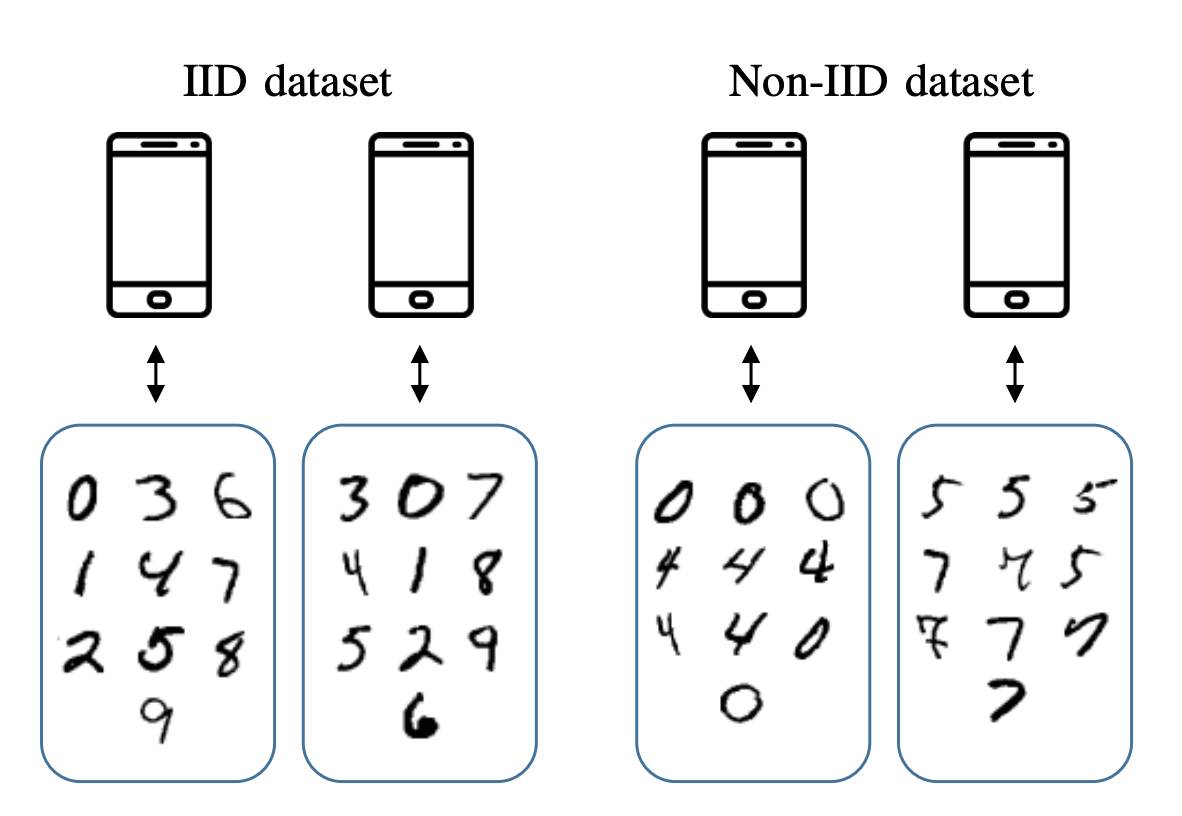
\includegraphics[scale=0.7]{../images/iid_vs_noniid.png}
    \caption{Minh họa kịch bản dữ liệu IID và Non-IID trên tập dữ liệu MNIST \cite{hellstrom2020wireless}}
    \label{fig:iid_noniid}
\end{figure}

% Mặt khác, nghiên cứu \cite{zhao2018federated} chỉ ra rằng \textbf{hệ thống FL có thể bị giảm hiệu quả nghiêm trọng khi làm việc trên dữ liệu Non-IID vì mô hình toàn cục không được huấn luyện trên các tập dữ liệu tuân theo phân phối đều}. 

Mặt khác, nghiên cứu \cite{zhao2018federated} chỉ ra rằng \textbf{hệ thống FL có thể bị giảm hiệu quả nghiêm trọng khi làm việc trên dữ liệu Non-IID. Nguyên nhân được chỉ ra là do đạo hàm trên từng lô (batch) dữ liệu không đại phỏng được đạo hàm trên toàn bộ dữ liệu}. Để hiểu rõ vấn đề mình đang đối mặt, dựa trên nghiên cứu \cite{zhu2021federated}, khóa luận tiến hành khảo sát bốn kịch bản về dữ liệu Non-IID: (1) - Phân phối thuộc tính khác nhau giữa các máy khách, (2) - Phân phối nhãn khác nhau giữa các máy khách, (3) - Phân phối thời gian khác nhau giữa các máy khách, (4) - Các kịch bản khác.

\subsection{Phân phối thuộc tính khác nhau giữa các máy khách}

Với kịch bản này, phân phối thuộc tính $p(x)$ trên các máy khách là đôi một khác nhau. Không gian thuộc tính của các máy khách có thể khác nhau hoàn toàn, trùng lặp một vài thuộc tính hoặc trùng lặp hoàn toàn.

Các hệ thống Vertical FL thường rơi vào trường hợp đầu tiên. Ví dụ, trong Hình \ref{fig:vertical_fl}, các thuộc tính mà máy khách 1 quản lý (\textit{Age, Height}) khác hoàn toàn với các thuộc tính tại máy khách 2 (\textit{Sex, Weight}) nhưng các thuộc tính này là của chung dữ liệu định danh (\textit{Person A, B, C,...}).

\begin{figure}[H]
    \centering
    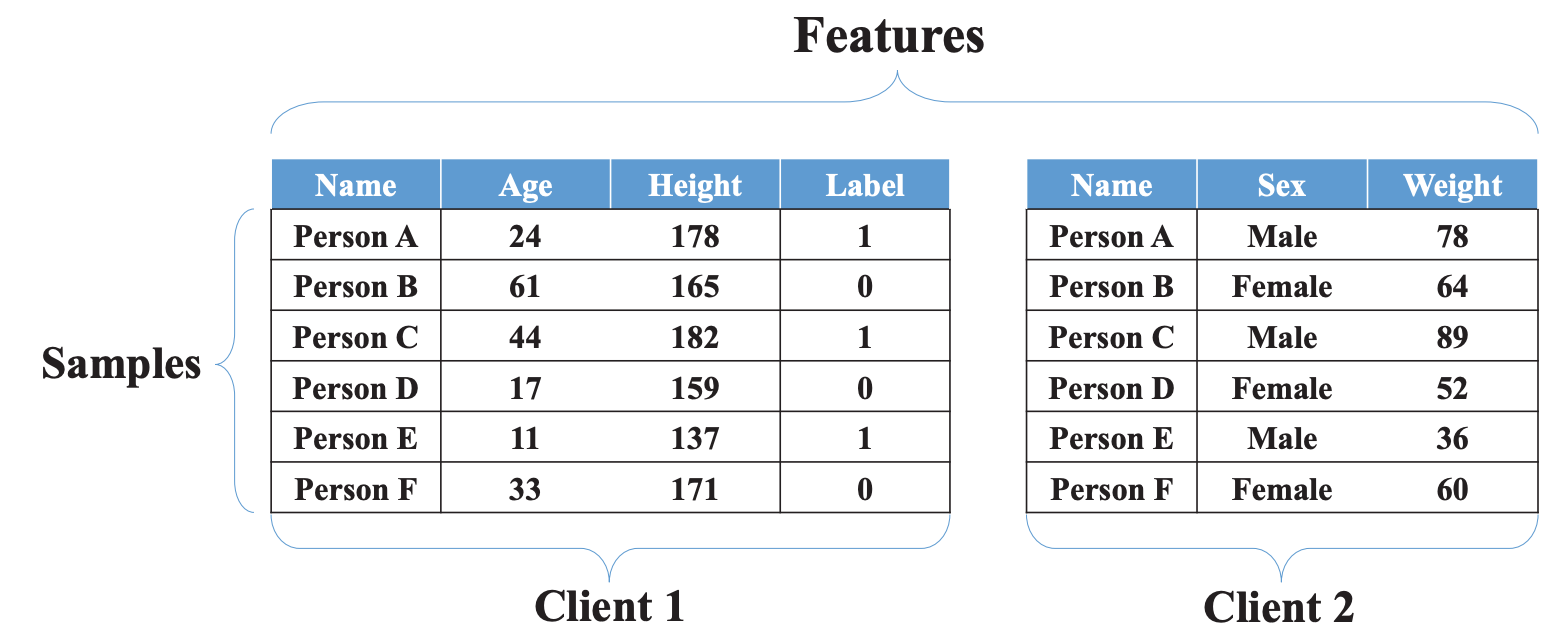
\includegraphics[scale=0.6]{../images/vertical_fl.png}
    \caption{Minh họa dữ liệu Non-IID trên thuộc tính \cite{zhu2021federated}}
    \label{fig:vertical_fl}
\end{figure}

Đối với trường hợp thứ hai, hai máy khách có thể cùng quản lý một số thuộc tính dữ liệu. Ví dụ, đối với dữ liệu của một hệ thống camera dám sát, hai camera bất kỳ có thể cùng lưu hình một người với các góc chụp khác nhau.

Trường hợp cuối chính là đặc điểm chính của hệ thống Horizontal FL. Tại đây, không gian thuộc tính của các máy khách là hoàn toàn giống nhau. Trong Hình \ref{fig:vertical_fl}, nếu máy khách 1 và máy khách 2 cùng quản lý các thuộc tính giống nhau và các mẫu dữ liệu chứa dữ liệu rất khác nhau (ví dụ máy khách 1 chứa tập người dùng trẻ tuổi, máy khách 2 chứa tập người dùng cao tuổi), thì đây là một ví dụ đơn giản cho trường hợp Non-IID này.

\subsection{Phân phối nhãn khác nhau giữa các máy khách}

Đây là trường hợp dữ liệu Non-IID phổ biến nhất, gây hại nghiêm trọng cho hệ thống FL \cite{zhu2021federated}, cũng chính là trường hợp mà khóa luận hướng tới giải quyết. Tại đây, phân phối nhãn của hai máy khách $c_i, c_j$ bất kỳ là khác nhau: $p_i(y) \ne p_j(y)$ và xác suất thuộc tính $x$ có nhãn dữ liệu $y$: $p(x|y)$ của các máy khách là như nhau. Một kịch bản thường thấy của trường hợp này được trình bày trong nghiên cứu \cite{mcmahan2017communication}: Mỗi máy khách sẽ chỉ chứa các điểm dữ liệu thuộc về $k$ nhãn (Hình \ref{fig:my_noniid}). Trong đó, $k$ là một siêu tham số biểu diễn độ mất cân bằng về nhãn. $k$ càng nhỏ, hệ thống mất cân bằng nhãn càng mạnh. Khóa luận này thiết đặt môi trường dữ liệu theo cách tương tự như vậy.

\begin{figure}[H]
    \centering
    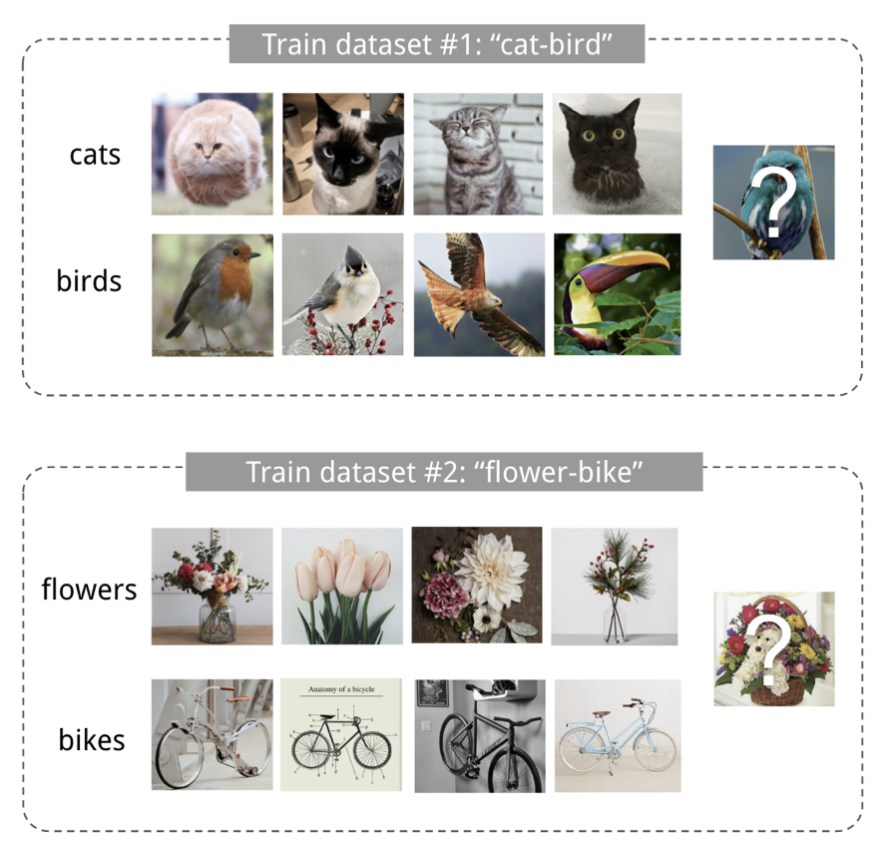
\includegraphics[scale=0.7]{../images/noniid_label.png}
    \caption{Minh họa dữ liệu Non-IID trên nhãn với của hai máy khách với $k=2$}
    \label{fig:my_noniid}
\end{figure}

Ngoài ra, còn một trường hợp phổ biến khác liên quan đến việc dữ liệu Non-IID trên nhãn. Đối với trường hợp này, xác suất thuộc tính $x$ được gán nhãn $y$: $p(y|x)$ là khác nhau giữa các máy khách. Ví dụ, với một bức ảnh trên mạng xã hội, người dùng $A$ có thể gán nhãn "yêu thích", trong khi người dùng $B$ gán nhãn "không yêu thích".

\subsection{Phân phối thời gian khác nhau giữa các máy khách}

Một ví dụ dễ hiểu cho trường hợp này là việc hai người dùng $c_i$, $c_j$ thu thập dữ liệu trong hai khoảng thời gian khác nhau. Dẫn đến việc phân phối $p_i(x, y|t) \ne p_j(x, y|t)$, với $t$ là một thời điểm nhất định. Một trường hợp khác của kịch bản này là phân phối $p(x, y|t)$ của một máy khách bị thay đổi liên tục theo thời gian. Ví dụ, một hệ thống camera giám sát có thể ghi nhận hình ảnh của rất nhiều người vào các ngày làm việc trong tuần nhưng lại có rất ít hình ảnh vào những ngày nghỉ.

\subsection{Các kịch bản khác}

Các kịch bản còn lại thường rơi vào hai trường hợp: (1) - Phân phối thuộc tính và nhãn là khác nhau giữa các máy khách, (2) - Số lượng dữ liệu huấn luyện là khác nhau giữa các máy khách.

\section{Tối ưu hệ thống Federated Learning trên dữ liệu Non-IID}

\subsection{Tối ưu dựa trên dữ liệu}

Việc mô hình toàn cục không được làm việc với dữ liệu tuân theo phân phối đều trên từng người dùng, mà thay vào đó là phân phối Non-IID, khiến cho hiệu suất hệ thống bị sụt giảm nghiêm trọng \cite{zhao2018federated}. Hướng tối ưu dựa trên dữ liệu trực tiếp giải quyết vấn đề này bằng hai cách: (1) - Chia sẻ dữ liệu, (2) - Tăng cường dữ liệu.

\textbf{Chia sẻ dữ liệu.} Chia sẻ dữ liệu \cite{zhu2021federated} được thực hiện bằng cách xây dựng một tập dữ liệu chứa dữ liệu của tất cả các nhãn theo phân phối đều. Dữ liệu trong tập này được thu thập trực tiếp từ các máy khách và gửi về máy chủ để kết hợp huấn luyện mô hình toàn cục.

\textbf{Tăng cường dữ liệu.} Cùng với ý tưởng cho phép mô hình toàn cục được học trên các tập dữ liệu có phân phối đều các nhãn trong hệ thống, tăng cường dữ liệu \cite{tanner1987calculation} nhằm mục đích gia tăng sự đa dạng của dữ liệu huấn luyện. Phương pháp này đòi hỏi các máy khách phải gửi phân phối dữ liệu của mình về máy chủ. Máy chủ theo đó yêu cầu các máy khách tạo ra ảnh mới \cite{duan2019astraea} với số lượng và nhãn lớp biết trước, hoặc tự mình tạo ra ảnh mới bằng cách sử dụng GAN \cite{zhu2021federated} để có thể huấn luyện trên một tập dữ liệu chứa tất cả các nhãn với phân phối trung bình.

Các phương pháp nêu trên đều giúp hệ thống FL "chống chịu" tốt trước dữ liệu Non-IID. Tuy nhiên, đỏi hỏi máy khách gửi thông tin cá nhân về máy chủ là vi phạm mục tiêu ban đầu của hệ thống FL - bảo vệ quyền riêng tư dữ liệu của người dùng.

\subsection{Tối ưu dựa trên thuật toán}

\subsubsection{Fine-tune cục bộ}

Thực hiện fine-tune, hay tinh chỉnh mô hình ở máy khách, là kỹ thuật mạnh mẽ trong việc cá nhân hóa mô hình học cho các tập dữ liệu riêng biệt. Kỹ thuật này hướng đến việc fine-tune mô hình học tại các máy khách sau khi nhận được mô hình từ máy chủ \cite{wang2019federated}.

Một hướng tiếp cận phổ biến được đề ra là sử dụng ML trong việc tạo ra một mô hình toàn cục tốt, có thể thích ứng với tập dữ liệu mới trên máy khách một cách nhanh chóng. Các thuật toán theo hướng này \parencite{chen2018federated, fallah2020personalized} sử dụng các kỹ thuật ML có khả năng tạo ra một khởi tạo tốt như \codeword{Model-Agnostic Meta-Learning (MAML)} \cite{finn2017model} hay \codeword{Meta-SGD} \cite{li2017meta} để huấn luyện mô hình toàn cục. Mô hình toàn cục này, trong quá trình chạy thực tế trên một máy khách mới, hoàn toàn có thể đạt hội tụ chỉ sau một hoặc một vài bước huấn luyện.

\subsubsection{Lớp cá nhân hóa}

Các thuật toán theo hướng này cho phép duy trì một phần của mạng học sâu trên máy khách. Cụ thể, thuật toán chia mạng học sâu thành hai thành phần: phần chung và phần riêng. Phần chung được hợp tác huấn luyện bởi các máy khách và được tổng hợp bởi máy chủ. Phần riêng tồn tại riêng biệt trên từng máy khách, được máy khách trực tiếp duy trì và huấn luyện.

\label{open_question}
Bằng các lớp cá nhân hóa, các thuật toán nêu trên đã giải quyết được sự khác nhau về dữ liệu giữa các máy khách, từ đó tránh được phần nào sự giảm hiệu suất trên dữ liệu Non-IID. Nhưng các lớp thuộc phần chung của mạng học sâu được huấn luyện theo thuật toán \codeword{FedAvg} nên vẫn có thể bị giảm hiệu suất rất lớn khi dữ liệu huấn luyện bị Non-IID nặng. \textbf{Vậy có thể làm gì để các lớp này có thể thích ứng nhanh với tập dữ liệu của máy khách chỉ sau một vài bước huấn luyện?}

\subsection{Tối ưu dựa trên hệ thống}

\subsubsection{Gom cụm người dùng}

Cách tiếp cận FL truyền thống giả định rằng hệ thống này chỉ bao gồm một máy chủ. Điều này làm cho việc học các đặc tính của tất cả các máy khách trong môi trường dữ liệu Non-IID là khó khả thi. Để giải quyết vấn đề này, một hệ thống huấn luyện với nhiều máy chủ được đề xuất. Câu hỏi đặt ra là: Làm sao để biết một máy khách nên huấn luyện cùng với máy chủ nào? 

Trong ngữ cảnh đa máy chủ, thuật toán \codeword{IFCA} \cite{ghosh2020efficient} trả lời câu hỏi trên bằng cách gửi trọng số của tất cả các máy chủ cho từng máy khách. Các máy khách theo đó tìm ra được trọng số cho độ lỗi nhỏ nhất trên tập dữ liệu cục bộ và gửi thông tin sau khi huấn luyện cục bộ của mình về máy chủ đó để cập nhật mô hình toàn cục. Việc gửi toàn bộ trọng số của các máy chủ đến một máy khách khiến cho thuật toán này tăng chi phí giao tiếp lên gấp $k$ lần, với $k$ là số lượng máy chủ của hệ thống.

Một cách khác để trả lời câu hỏi trên là đánh giá sự tương đồng của trọng số do máy khách gửi về \cite{zhu2021federated}. Một thang độ đo sự tương đồng như độ đo cosine được máy chủ sử dụng trên các trọng số của máy khách. Từ đó biết được nên tổng hợp trọng số của các máy khách nào với nhau.

Với việc lượng dữ liệu và thiết bị biên ngày càng tăng lên, việc duy trì nhiều máy chủ là thực sự cần thiết khi đối mặt với nhu cầu nâng cấp hệ thống học. Tuy nhiên, chi phí giao tiếp và phương pháp gom cụm vẫn là những vấn đề rất lớn cần giải quyết.

\section{Meta-Learning trong Federated Learning}

ML được áp dụng vào hệ thống FL như một phương pháp tối ưu thuộc nhóm "Fine-tune cục bộ". Các thuật toán ML được sử dụng trong hệ thống FL nhằm mục đích tạo ra một mô hình toàn cục tốt, giúp hội tụ nhanh trên tập dữ liệu phân bố trên các máy khách.

\subsection{Diễn giải Meta-Learning}

ML là một phương pháp học mới, cho phép mô hình học có thể gia tăng kinh nghiệm qua việc thực hiện nhiều nhiệm vụ khác nhau trong cùng một phân phối nhiệm vụ. Dẫn đến việc các mô hình ML có khả năng thích ứng nhanh trên nhiệm vụ mới chỉ sau một vài bước huấn luyện với dữ liệu huấn luyện giới hạn. Đây là một phát kiến quan trọng, đóng vai trò trong việc đưa cách học tập của máy trở nên tiệm cận với cách học tập của con người \cite{harlow1949formation}.

Đối với phương pháp huấn luyện mô hình học truyền thống, chúng ta huấn luyện mô hình dự đoán $\hat{y} = f_\theta(x)$ trên tập dữ liệu $\mathcal{D} = \{ (x_i, y_i)\}_{i=1}^{|\mathcal{D}|}$ của nhiệm vụ $T$ gồm các cặp thuộc tính và nhãn tương ứng. Ký hiệu $\mathcal{L}$ là hàm lỗi, $\omega$ là giả định ban đầu của hệ thống học, mục tiêu của việc học là tối thiểu hóa hàm lỗi trên tập dữ liệu $\mathcal{D}$ bằng cách tìm một bộ trọng số $w^*$ thỏa mãn:

\begin{equation}
    w^* = \arg \min_w \mathcal{L}(\mathcal{D}; w, \omega)
\end{equation}

Hướng tiếp cận của ML nằm ở chỗ cố gắng học một giả định ban đầu $\omega$ thật tốt. Điều này đạt được thông qua việc học một phân phối các nhiệm vụ $p(T)$ \cite{hospedales2020meta}. Sau khi học được một giả định ban đầu tốt, có thể áp dụng giả định này cho các nhiệm vụ mới trong cùng phân phối nhiệm vụ: $T \sim p(T)$.

Về mặt công thức, ký hiệu $\mathcal{L}(\mathcal{D}, \omega)$ là hàm lỗi biểu diễn sự hiệu quả việc sử dụng $\omega$ trong huấn luyện nhiệm vụ $T$ có tập dữ liệu $\mathcal{D}$, chúng ta có thể biểu diễn hàm mục tiêu của ML như sau:

\begin{equation}
    \min_{\omega} \mathop{\mathbb{E}}_{T\sim p(T)} \mathcal{L}(\mathcal{D}, \omega)
\end{equation}

Trong thực tế, người ta thực hiện mục tiêu trên bằng cách huấn luyện mô hình học trên tập dữ liệu $\mathcal{D}_{train} = \{(\mathcal{D}_{train(i)}^{support}, \mathcal{D}_{train(i)}^{query})\}_{i=1}^{|\mathcal{D}_{train}|}$ và kiểm thử trên tập dữ liệu $\mathcal{D}_{test} = \{(\mathcal{D}_{test(i)}^{support}, \mathcal{D}_{test(i)}^{query})\}_{i=1}^{|\mathcal{D}_{test}|}$. Mục tiêu của việc huấn luyện là tìm ra một giá trị $\omega^*$, sao cho khi sử dụng giá trị này trong huấn luyện một nhiệm vụ $T\sim p(T)$ thì đạt được hiệu quả cao:

\begin{dmath}
    \label{eq:meta_train}
    \omega^* = \arg \max_{\omega} \log{p(\omega|\mathcal{D}_{source})}
\end{dmath}

Trong quá trình kiểm thử, tham số $\omega^*$ được sử dụng trong việc huấn luyện mô hình giải quyết nhiệm vụ $T_{new}$: $w^* = \arg \max_{w} \log{p(w|\omega^*, \mathcal{D}_{test(new)}^{support})}$. Để đánh giá hiệu quả của việc sử dụng $\omega$ trong huấn luyện nhiệm vụ $T_{new}$, người ta dựa vào kết quả của $w^*$ trên tập $\mathcal{D}_{test(new)}^{query}$.

Để giải phương \ref{eq:meta_train}, nghiên cứu \cite{hospedales2020meta} nhìn nhận ML dưới góc độ một bài toán tối ưu hai cấp độ. Dưới góc nhìn này, phương trình \ref{eq:meta_train} được giải bằng cách đạt được mục tiêu tại hai cấp độ: (1) - Cấp độ thấp, (2) - Cấp độ cao.

Đối với cấp độ thấp, mục tiêu là giải quyết nhiệm vụ $T_i$ dựa vào $\omega$:

\begin{eqnarray}
    \label{eq:inner_opt}
    w^*_i(\omega) = \arg \min_{w} \mathcal{L}^{task} \left(w, \omega, \mathcal{D}_{train(i)}^{support}\right)
\end{eqnarray}

Bằng kỹ thuật SGD, phương trình \ref{eq:inner_opt} có lời giải sau:

\begin{equation}
    \label{sol:inner_opt}
    \begin{cases}
        w_{i(0)} = \omega\\
        w_{i(j)} = w_{i(j-1)} - \alpha \nabla \mathcal{L}^{task}\left(w_{i(j-1)}, \omega, \mathcal{D}_{train(i)}^{support}\right)
    \end{cases}
\end{equation}

Hay:

\begin{dmath}
    w_i \leftarrow w_i - \alpha\nabla\mathcal{L}^{task}(w_i)
\end{dmath}

Đối với cấp độ cao, mục tiêu là tìm ra tham số $\omega^*$ tối ưu, giúp việc học một nhiệm vụ mới $T_{new}\sim p(T)$ được thực hiện nhanh chóng và đạt hiệu suất cao:

\begin{eqnarray}
    \label{eq:outer_opt}
    \omega^* = \arg \min_{\omega} \sum_{i=1}^{|\mathcal{D}_{source}|} \mathcal{L}^{meta}\left(w^*_i(\omega), \omega, \mathcal{D}_{train(i)}^{query}\right)
\end{eqnarray}

Áp dụng kỹ thuật SGD, lời giải cần tìm cho phương trình \ref{eq:outer_opt} được biểu diễn như sau:

\begin{dmath}
    \begin{cases}
        \omega_0 = \Omega, \Omega \text{ là giá trị khởi tạo ngẫu nhiên}\\
        \omega_j = \omega_{j-1} - \beta \nabla \sum_{i=1}^{|\mathcal{D}_{source}|} \mathcal{L}^{meta}\left(w_i^*(\omega), \omega, \mathcal{D}_{train(i)}^{query}\right)
    \end{cases}
\end{dmath}

Hay:

\begin{dmath}
    \label{sol:outer_opt}
    \omega \leftarrow \omega - \beta\nabla \sum_{i=1}^{|\mathcal{D}_{source}|} \mathcal{L}^{meta}\left(w_i^*(\omega)\right)
        \leftarrow \omega - \beta\nabla \sum_{i=1}^{|\mathcal{D}_{source}|} \mathcal{L}^{meta}\left( w_i - \alpha\nabla\mathcal{L}^{task}(w_i)\right)
        \leftarrow \omega - \beta \sum_{i=1}^{|\mathcal{D}_{source}|} \left( I - \alpha \nabla^2 \mathcal{L}^{task}(w_i) \right) \times \nabla \mathcal{L}^{meta}\left( w_i - \alpha\nabla\mathcal{L}^{task}(w_i)\right)
\end{dmath}

\subsection{Tích hợp Meta-Learning vào Federated Learning}

% Hai phương trình \ref{eq:inner_opt} và \ref{eq:outer_opt} đặt trong tương quan với hai mục tiêu được trình bày trong phần \ref{purpose_fl}, có thể thấy rõ điểm tương đồng giữa hệ thống FL và hệ thống ML. Theo đó, các mục tiêu cấp thấp trong ML tương đồng với các mục tiêu cục bộ trong hệ thống FL, mục tiêu cấp cao trong hệ thống ML tương đồng với mục tiêu toàn cục của hệ thống FL. Từ đây, có thể dễ dàng kết hợp ML và FL bằng cách thay thế hệ hàm mục tiêu của hệ thống FL bằng hệ hàm mục tiêu của ML.

Nhìn nhận hai phương trình \ref{eq:inner_opt} và \ref{eq:outer_opt}, có thể thấy chúng dễ dàng đem thay thế các mục tiêu của một hệ thống FL truyền thống (được trình bày trong phần \ref{purpose_fl}). Theo đó, mục tiêu cấp thấp và cấp cao trong ML có thể lần lượt thay thế cho mục tiêu cục bộ và mục tiêu toàn cục trong hệ thống FL. Từ đây, có thể dễ dàng tích hợp ML vào hệ thống FL.

Thật vậy, nghiên cứu \cite{fallah2020personalized} đã tích hợp thuật toán \codeword{MAML} vào hệ thống FL và biểu diễn lại hàm mục tiêu toàn cục của hệ thống từ phương trình \ref{eq:opt_server} như sau:

\begin{equation}
    \label{eq:opt_meta_fl}
    \min_{w_G} f_{global}(w_G)
        =\min_{w_G} \frac{1}{n} \sum_{i=1}^n f_{local}\left(w_i - \alpha \nabla f_{local}(w_i, \mathcal{D}_{train(i)}^{support}), \mathcal{D}_{train(i)}^{query}\right)
\end{equation}

Trong hàm số \ref{eq:opt_meta_fl}, ta có thể nhận thấy sự xuất hiện của hai tập dữ liệu $\mathcal{D}_{train(i)}^{support}$ và $\mathcal{D}_{train(i)}^{query}$. Điều này có nghĩa là hệ thống FL huấn luyện theo hướng ML cần phải chia lại tập dữ liệu tại các máy khách theo kiểu ML. Một máy khách $c_i$ tham gia huấn luyện bao gồm hai tập dữ liệu $\mathcal{D}_{train(i)}^{support}$ và $\mathcal{D}_{train(i)}^{query}$. Trong quá trình kiểm thử, dữ liệu của máy khách $c_i$ cũng được chia thành hai tập $\mathcal{D}_{test(i)}^{support}$ và $\mathcal{D}_{test(i)}^{query}$. Trong đó, $c_i$ cần thực hiện fine-tune mô hình trên tập $\mathcal{D}_{test(i)}^{support}$ và đánh giá mô hình trên tập $\mathcal{D}_{test(i)}^{query}$.

Từ phương trình tổng hợp mô hình toàn cục bằng phương pháp lấy trung bình trọng số \ref{eq:agg_w}, áp dụng phương pháp SGD như trong phương trình \ref{sol:outer_opt}, phương trình tổng hợp mô hình toàn cục trong hệ thống FL tích hợp ML tại bước huấn luyện toàn cục thứ $t$ có dạng:

\begin{dmath}
    \label{eq:agg_fedmeta}
    w_G^{t+1} = \sum_{i=1}^n{\frac{n_i}{N} w_i^{t+1}}
        = \sum_{i=1}^n{\frac{n_i}{N}\left[ w_i^t - \beta \left( I - \alpha \nabla^2 f_{local}(w_i^t) \right) \times \nabla f_{local}\left( w_i^t - \alpha\nabla f_{local}(w_i^t)\right) \right]}
\end{dmath}

Ngoài thuật toán \codeword{MAML}, các thuật toán ML theo hướng tối ưu hai cấp độ đều có thể dễ dàng tích hợp vào hệ thống FL. Ví dụ, nghiên cứu \cite{chen2018federated} đã tích hợp thuật toán \codeword{Meta-SGD} vào hệ thống FL của họ. Tương tự như \codeword{MAML}, \codeword{Meta-SGD} được cấu trúc theo hướng tối ưu hai cấp độ. Tuy nhiên, có một thay đổi nhỏ giúp thuật toán này đạt độ chính xác cao hơn \codeword{MAML}: thuật toán coi siêu tham số học $\alpha$ là một tham số có thể học, được cấu hình dưới dạng một mảng có kích thước bằng trọng số mô hình và được tối ưu trong mục tiêu cấp cao.

Tóm lại, cả hai nghiên cứu \parencite{chen2018federated, fallah2020personalized} đã chứng minh được việc tích hợp ML vào hệ thống FL giúp đạt hiệu quả cao hơn \codeword{FedAvg} về độ chính xác trên cả hai phương diện lý thuyết và thực nghiệm. \textbf{Nhờ vào khởi tạo tốt sinh ra bởi các thuật toán ML, mô hình toàn cục có khả năng thích ứng nhanh hơn trên tập dữ liệu mới, từ đó hội tụ nhanh, tính cá nhân hóa cho từng người dùng và độ chính xác thu được đạt kết quả cao hơn} \codeword{FedAvg} \textbf{khi làm việc trên dữ liệu Non-IID}.

\section{Personalization Layer trong Federated Learning}

Khóa luận tiến hành khảo sát kết quả của các kỹ thuật tối ưu hệ thống FL trên dữ liệu Non-IID và nhận thấy các thuật toán theo hướng PL đạt kết quả rất cao và có tiềm năng phát triển thêm (Bảng \ref{tab:acc_paper}). Các thuật toán theo hướng này chia mạng học sâu ra làm hai phần \cite{zhu2021federated}: phần chung và phần riêng. Theo đó, phần chung được hợp tác huấn luyện bởi tất cả các máy khách trong hệ thống còn phần riêng được từng máy khách huấn luyện riêng biệt trên tập dữ liệu cục bộ. \textbf{Chính nhờ việc các lớp học sâu trong phần riêng nắm bắt tốt các đặc trưng của từng tập dữ liệu riêng biệt, đã làm cho cách tiếp cận này trở nên mạnh mẽ trên dữ liệu có tính cá nhân hóa cao như dữ liệu Non-IID}.

\begin{table}[H]
    \centering
    \caption{Độ chính xác (\%) của các hệ thống FL trên dữ liệu Non-IID của tập dữ liệu CIFAR-10 \cite{shamsian2021personalized}. Các thuật toán PL được in đậm.}
    \label{tab:acc_paper}
    \resizebox{\linewidth}{!}{%
    \begin{tabular}{c|ccc} 
    \toprule
    \diagbox{Thuật toán}{\#clients} & 10           & 50           & 100           \\ 
    \midrule
    Per-FedAvg                      & 76.65 ± 4.84 & 83.03 ± 0.25 & 80.19 ± 1.99  \\
    \textbf{FedPer}                 & 87.27 ± 1.39 & 83.39 ± 0.47 & 80.99 ± 0.71  \\
    pFedMe                          & 87.69 ± 1.93 & 86.09 ± 0.32 & 85.23 ± 0.58  \\
    \textbf{LG-FedAvg}              & 89.11 ± 2.66 & 85.19 ± 0.58 & 81.49 ± 1.56  \\
    \bottomrule
    \end{tabular}
    }
\end{table}

Một thuật toán điển hình theo hướng tiếp cận này là \codeword{FedPer} \cite{arivazhagan2019federated}. \codeword{FedPer} quy định phần chung của mạng học sâu là các lớp rút trích đặc trưng, phần riêng của mạng là các lớp còn lại. Tác giả của \codeword{FedPer} đã thực hiện nhiều thí nghiệm chứng tỏ rằng thuật toán này đạt điệu quả cao hơn nhiều so với \codeword{FedAvg} khi làm việc trên dữ liệu Non-IID.

Thuật toán \codeword{LG-FedAvg} \cite{liang2020think} cũng được xếp vào nhóm thuật toán sử dụng lớp cá nhân hóa. Tuy nhiên, ngược lại với \codeword{FedPer}, \codeword{LG-FedAvg} chỉ định phần riêng là các lớp rút trích đặc trưng trong mạng học sâu. Thực nghiệm cho thấy, \codeword{LG-FedAvg} đạt hiệu quả tốt hơn \codeword{FedAvg} trên cả các máy khách sẵn có trong hệ thống lẫn các máy khách chỉ vừa mới tham gia hệ thống.

Tuy nhiên, như câu hỏi về các cải thiện các trọng số phần chung đã được nêu ra trong phần \ref{open_question}, hiệu suất của hệ thống FL cài đặt theo hướng PL vẫn có thể được cải thiện vì các lớp phần chung chưa thực sự mạnh mẽ và còn phụ thuộc nhiều vào phân phối dữ liệu. Cụ thể, các lớp phần chung này được huấn luyện bằng thuật toán \codeword{FedAvg} nên có thể gặp tình trạng tương tự như \codeword{FedAvg} do phân bố dữ liệu không đồng đều trong kịch bản Non-IID. Do đó, cần cải thiện cách huấn luyện của các lớp học sâu trong phần chung để chúng bớt phụ thuộc vào dữ liệu hơn. Nói cách khác, các lớp này cần có khả năng làm việc khách quan, "đối xử" công bằng hơn với các tập dữ liệu trên máy khách.

% Như đã thảo luận trước đó, các thuật toán ML có khả năng thích ứng nhanh trên tập dữ liệu mới thông qua việc học nhiều nhiệm vụ khác nhau. Hơn nữa, dựa vào phân tích tính tương đồng về hệ hàm mục tiêu của FL và ML ở trên, ta có thể coi các nhiệm vụ khác nhau của ML chính là các máy khách trong hệ thống FL. Do đó, khóa luận sử dụng phương pháp huấn luyện mô hình của ML vào huấn luyện các lớp phần chung nhằm thu được các lớp phần chung có khả năng trở thành một khởi tạo tốt dựa vào dữ liệu huấn luyện và thích ứng nhanh trên dữ liệu kiểm tra.

% Hai thuật toán điển hình theo hướng PL là \codeword{FedPer} \cite{arivazhagan2019federated} và \codeword{LG-FedAvg} \cite{liang2020think}. Trong phần này, hai thuật toán trên được phân tích và đưa ra các nhận xét về ưu, nhược điểm của từng thuật toán. Từ đó kết hợp chúng với các thuật toán \codeword{FedMeta}.
